%
% electromagnetic_wave_2.tex -- Bild zum Thema Optische Fourier-Transformation <opt>
%
% (c) 2023 Marco Niederberger, Yanick Schoch; OST Ostschweizer Fachhochschule
%

% Inspiration: https://wiki.physik.uzh.ch/cms/latex:tikz:electromagnetic_wave
\documentclass[tikz]{standalone}
\usepackage{times}
\usepackage{tikz,tikz-3dplot}
\usepackage{pgfplots}
\usetikzlibrary{calc}
\usepackage{amsmath}
\usepackage{xcolor}

\pgfplotsset{compat=1.16}
\def\skala{1}

%
% opt_common.tex -- Commands and color definition for the paper <opt>
%
% (c) 2023 Marco Niederberger, Yanick Schoch; OST Ostschweizer Fachhochschule
%

%%% NEW COMMANDS %%%

% Lense (x, height, curvature)
\newcommand{\lense}[3]{
    \def\curvature{0.2}
    \path[fill=glass, draw=black, line width = 0.6, opacity=0.8] (#1,-#2) .. controls (#1 - #3,0) .. (#1,#2) .. controls (#1 + #3,0) .. (#1,-#2);
}

% Dimension arrow (xStart, xEnd, yHeight, text)
\newcommand{\optMeasurement}[4]{%
    \draw[<->] (#1, #3)--(#2, #3) node[above,midway] {#4};
}

% Annotated point
\newcommand{\point}[3]{
    \draw[fill=black] (#1) circle (1pt) node[#3] {#2};
}

%%% COLORS %%%

% Define Color
\definecolor{glass}{cmyk}{0.2,0,0,0}
\colorlet{optBlue}{blue!70!black}
\colorlet{optRed}{red!90!black}
\colorlet{optGreen}{green!50!black}

%%% STYLES %%%

% Laser rays
\tikzset{red ray/.style = {optRed, line width = 0.6}}
\tikzset{ray arrow/.style = {red ray, postaction=decorate,decoration={markings,mark=at position 0.52 with \arrow{stealth}}}}

\newcommand{\electromagneticWave}{
    \def\A{1.5}
    \def\nNodes{5}
    \def\nVectorsPerNode{2}
    \def\N{\nNodes*40}
    \def\xmax{\nNodes*pi/2*1.01}
    \pgfmathsetmacro\nVectors{(\nVectorsPerNode+1)*\nNodes}

    % draw E node and vector with some offset
    \def\drawENode{
        \draw[optGreen,thick,variable=\t,domain=\iOffset*pi/2:(\iOffset+1)*pi/2*1.01,samples=40]
        plot (\t,{\A*sin(\t*360/pi)},0);
        \foreach \k [evaluate={\t=\k*pi/2/(\nVectorsPerNode+1); \angle=\k*90/(\nVectorsPerNode+1);}]
            in {1,...,\nVectorsPerNode}{\draw[->, thin,optGreen!50]  (\iOffset*pi/2+\t,0,0) -- ++(0,{\A*sin(2*\angle+\iOffset*180)},0);
        }
    }

    % draw B node and vectors with some offset
    \def\drawBNode{
        \draw[optBlue,thick,variable=\t,domain=\iOffset*pi/2:(\iOffset+1)*pi/2*1.01,samples=40]
        plot (\t,0,{\A*sin(\t*360/pi)});
        \foreach \k [evaluate={\t=\k*pi/2/(\nVectorsPerNode+1); \angle=\k*90/(\nVectorsPerNode+1);}]
            in {1,...,\nVectorsPerNode}{\draw[->, thin,optBlue!50]  (\iOffset*pi/2+\t,0,0) -- ++(0,0,{\A*sin(2*\angle+\iOffset*180)});
        }
    }

    % main axes
    \draw[->, thin] (0,0,0) -- ++(\xmax*1.1,0,0) node[below left] {$z$};
    \draw[->, thin] (0,-\A*1.4,0) -- (0,\A*1.4,0) node[right] {$x$};
    \draw[->, thin] (0,0,-\A*1.4) -- (0,0,\A*1.4) node[below right] {$y$};

    % small axes
    \def\xOffset{{(\nNodes-2)*pi/2}}
    \def\yOffset{\A*1.2}
    \def\zOffset{\A*1.2}
    \draw[->, thin,black] (\xOffset,\yOffset,-\zOffset) -- ++(\A*0.6,0,0) node[right,align=center] {$S$};
    \draw[->, thin,optGreen]  (\xOffset,\yOffset,-\zOffset) -- ++(0,\A*0.6,0) node[right] {$E$};
    \draw[->, thin,optBlue]   (\xOffset,\yOffset,-\zOffset) -- ++(0,0,\A*0.6) node[above left] {$H$};

    % draw (anti-)nodes
    \foreach \iNode [evaluate={\iOffset=\iNode-1;}] in {1,...,\nNodes}{
        \ifodd\iNode \drawBNode \drawENode % E overlaps B
        \else        \drawENode \drawBNode % B overlaps E
        \fi
    }
}


\begin{document}
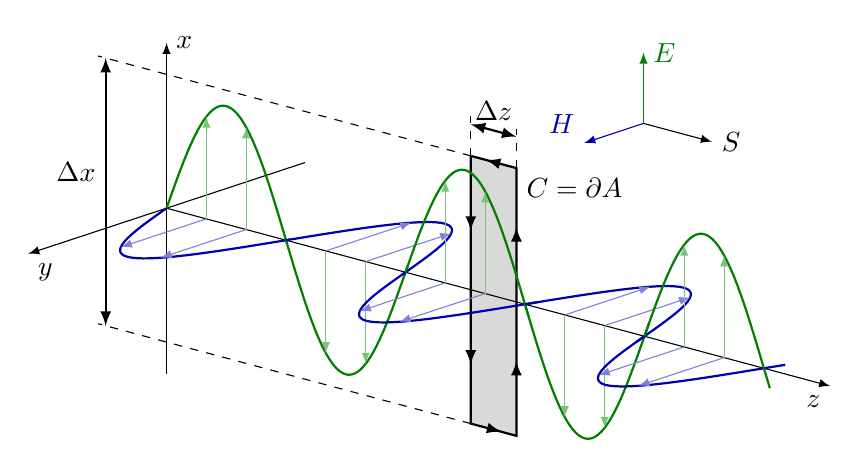
\begin{tikzpicture}[>=latex, thick, scale=\skala, x=(-15:1.0), y=(90:1.0), z=(-150:1.0)]
    % rectangle
    \def\xRectangle{4}
    \def\xRectangleWidth{0.6}
    \def\yRectangle{1.7}

    \fill[gray!30] (\xRectangle,\yRectangle,0) -- ++(\xRectangleWidth,0,0) -- ++(0,-2*\yRectangle,0) -- ++(-\xRectangleWidth,0,0);
    \draw[] (\xRectangle,\yRectangle,0) -- ++(\xRectangleWidth,0,0) node[below right]{$C=\partial A$}-- ++(0,-2*\yRectangle,0) -- ++(-\xRectangleWidth,0,0) -- (\xRectangle,\yRectangle,0);

    \draw[->] (\xRectangle,\yRectangle/2,0) -- ++(0,-0.1,0);
    \draw[->] (\xRectangle,-\yRectangle/2,0) -- ++(0,-0.1,0);
    \draw[->] (\xRectangle+\xRectangleWidth,\yRectangle/2,0) -- ++(0,0.1,0);
    \draw[->] (\xRectangle+\xRectangleWidth,-\yRectangle/2,0) -- ++(0,0.1,0);
    \draw[->] (\xRectangle+\xRectangleWidth/2,\yRectangle,0) -- ++(-0.1,0,0);
    \draw[->] (\xRectangle+\xRectangleWidth/2,-\yRectangle,0) -- ++(0.1,0,0);

    \draw[-, thin, dashed] (\xRectangle,\yRectangle,0) -- (-0.9,\yRectangle,0);
    \draw[-, thin, dashed] (\xRectangle,-\yRectangle,0) -- (-0.9,-\yRectangle,0);
    \draw[-, thin, dashed] (\xRectangle,\yRectangle,0) -- ++(0,0.5,0);
    \draw[-, thin, dashed] (\xRectangle+\xRectangleWidth,\yRectangle,0) -- ++(0,0.5,0);

    \draw[<->] (-0.8,\yRectangle,0) -- ++(0,-2*\yRectangle,0) node[anchor=south east, midway]{$\Delta x$};
    \draw[<->] (\xRectangle,\yRectangle+0.4,0) -- ++(\xRectangleWidth,0,0) node[anchor=south, midway]{$\Delta z$};

    \electromagneticWave
\end{tikzpicture}
\end{document}
